\documentclass{beamer}

\usetheme{CambridgeUS}
\usecolortheme{dolphin}

\usefonttheme{serif}
\usepackage{tikz}
\useinnertheme{rectangles}
\useoutertheme{miniframes}

\setbeamercolor*{mini frame}{fg=black,bg=white}
\setbeamercolor{section in head/foot}{fg=black, bg=white}


% Define colors
\definecolor{myblue}{RGB}{0, 102, 204}
\definecolor{mygreen}{RGB}{0, 153, 0}

\setbeamercolor{structure}{fg=myblue} % Color of text elements
\setbeamercolor{alerted text}{fg=mygreen} % Color of alerted text (e.g., \alert{})
\setbeamercolor{block title}{bg=myblue,fg=white} % Color of block titles
\setbeamercolor{block body}{bg=gray!5} % Color of block body
\setbeamercolor{block title alerted}{bg=mygreen,fg=white} % Color of block titles
\setbeamercolor{block body alerted}{bg=gray!5} % Color of block body
\setbeamercolor{itemize item}{fg=myblue} % Color of itemize bullets
\setbeamercolor{itemize subitem}{fg=mygreen} % Color of sub-itemize bullets
\setbeamercolor{enumerate item}{fg=myblue} % Color of enumerate bullets
\setbeamercolor{enumerate subitem}{fg=mygreen} % Color of sub-enumerate bullets
\setbeamercolor{title}{fg=myblue} % Color of title
\setbeamercolor{author}{fg=black} % Color of author
\setbeamercolor{date}{fg=black} % Color of date






% Declare lengths

\newlength{\leafnodewidth} 
\newlength{\leafnodeheightone} 
\newlength{\leafnodeheighttwo}
\newlength{\leafnodetextstart}
\newlength{\leafnodetextend}

\newlength{\internalnoderadius}

\newlength{\leveldistance}

% Set length values

\setlength{\leafnodewidth}{6mm}
\setlength{\leafnodeheightone}{3mm}
\setlength{\leafnodeheighttwo}{9mm} 

\setlength{\leafnodetextstart}{11mm}
\setlength{\leafnodetextend}{15mm}

\setlength{\internalnoderadius}{3.5mm}

\setlength{\leveldistance}{14mm}

% Declare colors
\definecolor{leafcolorone}{RGB}{255,0,0} % red
\definecolor{leafcolortwo}{RGB}{0,0,255} % blue
\definecolor{internalnodecolor}{RGB}{0,255,0} % green
\definecolor{highlightededgecolor}{RGB}{139,1,102} %dark magenta
\definecolor{codecolorone}{RGB}{139,1,102} %dark magenta
\definecolor{codecolortwo}{RGB}{45, 141, 38} % dark green
\definecolor{dimcolor}{RGB}{217, 217, 217}

%\addtobeamertemplate{navigation symbols}{}{%
%	\usebeamerfont{footline}%
%	\usebeamercolor[fg]{footline}%
%	\hspace{1em}%
%	\insertframenumber/\inserttotalframenumber
%}

% Define the \leafnode command
\newcommand{\leafnode}[6]{
	\begin{tikzpicture}
		\filldraw[color=#1!90, fill=#1!3, thick, font=\tiny] (0,0) rectangle (\leafnodewidth, -\leafnodeheightone) node[midway, text=#3] {#4};
		\filldraw[color=#2!90, fill=#2!3, thick, font=\small] (0,-\leafnodeheightone) rectangle (\leafnodewidth, -\leafnodeheighttwo) node[midway, text=#3] {#5};
		
		% the following portion is only for showing after demonstration
		
		%\filldraw[color=white!100, fill=white!100, thick, font=\scriptsize] (0,-\leafnodetextstart) rectangle (\leafnodewidth, -\leafnodetextend) node[midway, text=#3] {#6};
		
	\end{tikzpicture}
}


% Define the \leafnode command
\newcommand{\labelledleafnode}[6]{
	\begin{tikzpicture}
		\filldraw[color=#1!90, fill=#1!3, thick, font=\tiny] (0,0) rectangle (\leafnodewidth, -\leafnodeheightone) node[midway, text=#3] {#4};
		\filldraw[color=#2!90, fill=#2!3, thick, font=\small] (0,-\leafnodeheightone) rectangle (\leafnodewidth, -\leafnodeheighttwo) node[midway, text=#3] {#5};
		
		\filldraw[color=violet!100, fill=white!100, thick, font=\scriptsize] (0,-\leafnodetextstart) rectangle (\leafnodewidth, -\leafnodetextend) node[midway, text=#3] {#6};
		
	\end{tikzpicture}
}

% Define the \internalnode command with a color argument
\newcommand{\internalnode}[3]{
	\begin{tikzpicture}
		\filldraw[color=#1!90, fill=#1!5, thick, font=\scriptsize] (0,0) circle (\internalnoderadius) node[midway, text=#2] {#3};
	\end{tikzpicture}
}


% Minimum Indicator
\newcommand{\mindicator}[0]{
	
	\vspace{0.5mm}
	
	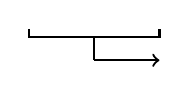
\begin{tikzpicture}
		
		\draw[black, thick] (0,0.1) -- (0,0) -- (1.66,0) -- (1.66,0.1);
		\draw[black, thick] (0.83,0) -- (0.83,-0.3);
		\draw[black, thick, ->] (0.83,-0.3) -- (1.66,-0.3);
		% Adding a dummy line for better positioning of the text
		\draw[white] (0,-0.4) -- (1.66,-0.4);
		
	\end{tikzpicture}
	\footnotesize{Minimum-weighted two nodes. Now these will be combined\ldots}
	% \begin{tikzpicture}
		% \node[draw=white, fill=white, rectangle, font=\footnotesize] at (0,0) {Minimum};
		% \end{tikzpicture}
	
}



\title{Huffman Coding}
\author[Anik \and Kowshik \and Jaber]{
	Section: A1 \\\and
	Group: 1\\ \and
	2005001-Anik Saha\\ \and 
	2005006-Kowshik Saha Kabya\\ \and 
	2005023-Jaber Ahmed Deedar}
\institute[CSE, BUET]{
	Department of CSE\\ 
	Bangladesh University of Engineering and Technology
}
\date{\today}


\begin{document}
\maketitle
	
	
	
	\tikzstyle{level 1} = [sibling distance=38mm]
	\tikzstyle{level 2} = [sibling distance=30mm]
	\tikzstyle{level 3} = [sibling distance=19mm]
	\tikzstyle{visible_edge} = [->, draw, leafcolortwo, thick]
	\tikzstyle{edge from parent} = [draw, teal, thick]
	\tikzstyle{emph} = [edge from parent/.style={->,highlightededgecolor,draw,ultra thick}]
	\tikzstyle{norm} = [edge from parent/.style={draw, teal, thin}]
	\tikzstyle{noedge} = [edge from parent/.style={draw, white, thin}]
	
	\tikzstyle{every node} = [inner sep=0]
	
	%Introduction
	\section{Introduction}
	
	\begin{frame}{What is Huffman Coding?}
		\begin{block}{Huffman Coding}
			Huffman coding is an efficient method of compressing data without losing information. 
			It provides an efficient, unambiguous code by analyzing the frequencies that certain symbols appear in a message. The algorithm is named after David A. Huffman, who developed it while he was a Sc.D student at MIT.
		\end{block}
	\end{frame}
	
	\begin{frame}{A little bit of History}
		
		{\small
			In 1951, Professor Robert M. Fano assigned a term paper on the problem of finding the most efficient binary code. In his paper, David A. Huffman developed an algorithm where he assigned shorter codes to the most frequently occurring characters and longer codes to the less frequently occurring characters, thus employing a variable-length encoding system.
		}
		
		\begin{center}
			\begin{tabular}{c c c}
				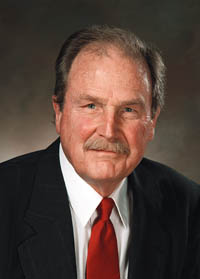
\includegraphics[height = 0.7in, width = 0.65in]{images/huffman.jpg} & 
				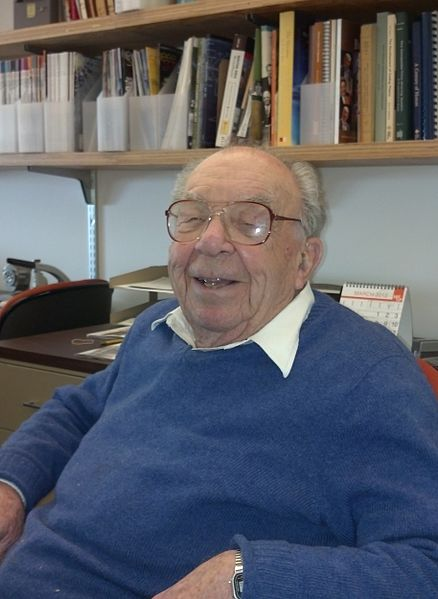
\includegraphics[height = 0.7in, width = 0.65in]{images/fano.jpg} & 
				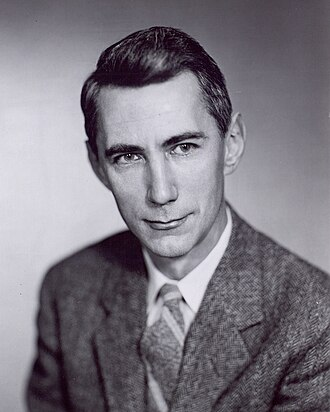
\includegraphics[height = 0.7in, width = 0.65in]{images/shannon.jpg} \\
				\scriptsize{David A. Huffman} & \scriptsize{Robert M. Fano} & \scriptsize{Claude Shannon} \\
			\end{tabular}    
		\end{center}
		
		{\small
			In doing so, Huffman outdid Fano, who alongside Claude Shannon developed a similar method. Huffman's bottom-up approach turned out to be more optimal than the top-down approach of Shannon and Fano.}
	\end{frame}
	
	\begin{frame}{Where is Huffman Coding used?}
		Huffman coding is used in various applications where data compression is necessary. Some of those applications are: 
		
		\begin{itemize}
			\item<1-> \textbf{File Compression:} ZIP, gzip, and zlib
			\item<2-> \textbf{Text Compression:} ASCII compression, HTML compression
			\item<3-> \textbf{Image Compression:} Entropy encoding in JPEG, image data compression in PNG
			\item<4-> \textbf{Audio Compression:} MP3, AAC
			\item<5-> \textbf{Network Communication:} Reduction of the size of data packets transmitted over networks
		\end{itemize}
	\end{frame}
	
	\begin{frame}{What's our objective?}
		
		\begin{block}{The Problem}
			Efficient digital communication requires converting any type of information into binary strings. Since resource is limited, we must find out a way of conversion such that the message requires least possible bandwidth to transmit.
		\end{block}
		\onslide<2->
		\begin{alertblock}{Our Goal}
			Now we look forward to finding an encoding scheme that requires minimum binary characters on average to encode a message.
		\end{alertblock}
		
	\end{frame}
	
	\begin{frame}{A Naive Solution}
		
		\onslide<1->
		\begin{alertblock}{}
			Let's assume, the alphabet consists of the letters A, B, C, D, and E.
		\end{alertblock}
		
		\onslide<2->
		\begin{block}{}
			Since there are 5 characters, we need at least 3 bits to uniquely encode each of them. So, we may randomly assign 3-bit binary strings from \textbf{000} to \textbf{100}
		\end{block}
		
	\end{frame}
	
	\begin{frame}{A Naive Solution}
		
		\begin{alertblock}{}
			Let's assume, the alphabet consists of the letters A, B, C, D, and E.
		\end{alertblock}
		
		\begin{block}{}
			Since there are 5 characters, we need at least 3 bits to uniquely encode each of them. So, we may randomly assign 3-bit binary strings from \textbf{000} to \textbf{100}
		\end{block}
		
		Doing so, we obtain the following table.
		
		\begin{table}
			\begin{tabular}{c|c}
				\hline
				\onslide<1-> \textbf{Letter} & \textbf{Binary Code} \\
				\hline
				A & 000  \\
				%				\hline
				B & 001  \\
				%				\hline
				C & 010 \\
				%				\hline
				D & 011 \\
				%				\hline
				E & 100 
				%				\hline
			\end{tabular}
		\end{table}
		
	\end{frame}
	
	\begin{frame}{A Naive Solution}
		
		\begin{table}
			\begin{tabular}{c|c}
				\hline
				\onslide<1-> \textbf{Letter} & \textbf{Binary Code} \\
				\hline
				A & 000  \\
				%				\hline
				B & 001  \\
				%				\hline
				C & 010 \\
				%				\hline
				D & 011 \\
				%				\hline
				E & 100 
				%				\hline
			\end{tabular}
		\end{table}
		
		\begin{block}
			
			\begin{itemize}
				\item Each of the letters needs 3 bits to encode.
				\item Therefore, if the length of a message = $n$, the expected length of the binary code = $3n$
			\end{itemize}
			
		\end{block}
		
	\end{frame}
	
	\begin{frame}{We Can Do Better\ldots}
		
		\begin{block}{}
			\centering
			Here, as a saviour, arrives the ingenious idea of Huffman
		\end{block}
		
	\end{frame}
	
	
	
	
	\section{Algorithm}
	
	\begin{frame}{Huffman's Idea}
		
		\onslide<1->
		\begin{block}{The Observation}
			
			\begin{itemize}
				
				\item Assigning shorter codes for more-frequent characters decreases the average length of the encoded message
				
			\end{itemize}
			
		\end{block}
		
	\end{frame}
	
	\begin{frame}{Huffman's Idea}
		
		\begin{alertblock}{A Greedy Algorithm}
			
			\begin{enumerate}
				\item Maintain a min-heap of nodes for characters with their relative frequencies as weights. For instance, a character with relative frequency 17\%, its weight is 0.17
				
				\item Pop two nodes with minimum weights 
				
				\item Merge them into a single node whose weight will be the summation of the previous nodes
				
				\item Push the newly created node back into the min-heap
				
				\item Repeat until the min-heap contains only the root of the tree
				
				\item Use the Huffman tree to encode any message
				
			\end{enumerate}
			
		\end{alertblock}
		
	\end{frame}
	
	\begin{frame}{Why Greedy Technique Works in Huffman Coding}
		
		\begin{block}{The Intuition Behind}
			\begin{itemize}
				\item The greedy approach always places more-frequent characters closer to the root of the tree
				
				\item This ensures that shorter codes are assigned to more-frequent characters and vice versa
				
			\end{itemize}
		\end{block}
	\end{frame}
	
	\begin{frame}{The Huffman Tree}
		\begin{alertblock}{Huffman Tree}
			In Huffman encoding, symbols are represented by nodes in a binary tree structure. It is built using bottom-up greedy approach.
		\end{alertblock}
	\end{frame}
	
	
	\section{Construction}
	
	
	% Construction of Huffman Tree
	
	
	% Frame 1 - Only leaf nodes
	\begin{frame}[c]{Construction of Huffman Tree}
		
		\leafnode{leafcolorone}{leafcolortwo}{black}{0.15}{D}{010}
		\leafnode{leafcolorone}{leafcolortwo}{black}{0.16}{E}{011}
		\leafnode{leafcolorone}{leafcolortwo}{black}{0.17}{A}{000}
		\leafnode{leafcolorone}{leafcolortwo}{black}{0.17}{C}{001}
		\leafnode{leafcolorone}{leafcolortwo}{black}{0.35}{B}{1}
		
		\onslide<2->
		\mindicator
		
	\end{frame} 
	
	
	
	% Frame 2 - One merge
	\begin{frame}[c]{Construction of Huffman Tree}
		
		\onslide <2>
		\leafnode{leafcolorone}{leafcolortwo}{black}{0.17}{A}{000}
		\leafnode{leafcolorone}{leafcolortwo}{black}{0.17}{C}{001}
		\internalnode{internalnodecolor}{black}{0.31}
		\leafnode{leafcolorone}{leafcolortwo}{black}{0.35}{B}{1}
		
		\mindicator
		
		\onslide <1->
		
		\begin{figure}
			
			\begin{tikzpicture}[
				level distance=\leveldistance
				]
				
				\node {\internalnode{white}{white}{1.00}}
				child[noedge]{
					node {\internalnode{white}{white}{0.65}}
					child[noedge]{
						node {\internalnode{white}{white}{0.34}}
						child[noedge]{
							node {\leafnode{white}{white}{white}{0.17}{A}{000}}
						}
						child[noedge]{
							node {\leafnode{white}{white}{white}{0.17}{C}{001}}
						}
					}
					child[noedge]{
						node {\internalnode{internalnodecolor}{black}{0.31}}
						child[norm]{
							node {\leafnode{leafcolorone}{leafcolortwo}{black}{0.15}{D}{010}}
						}
						child[norm]{
							node {\leafnode{leafcolorone}{leafcolortwo}{black}{0.16}{E}{011}}
						}
					}
				}
				child[noedge]{
					node {\leafnode{white}{white}{white}{0.35}{B}{1}}
				};
				
			\end{tikzpicture}
			
		\end{figure}
		
		
	\end{frame}
	
	
	
	
	% Frame 3 - Two merges
	\begin{frame}[c]{Construction of Huffman Tree}
		
		\onslide <2>
		\internalnode{internalnodecolor}{black}{0.31}
		\internalnode{internalnodecolor}{black}{0.34}
		\leafnode{leafcolorone}{leafcolortwo}{black}{0.35}{B}{1}
		
		\mindicator
		
		\onslide <1->
		\begin{figure}
			
			\begin{tikzpicture}[
				level distance=\leveldistance
				]
				
				\node {\internalnode{white}{white}{1.00}}
				child[noedge]{
					node {\internalnode{white}{white}{0.65}}
					child[noedge]{
						node {\internalnode{internalnodecolor}{black}{0.34}}
						child[norm]{
							node {\leafnode{leafcolorone}{leafcolortwo}{black}{0.17}{A}{000}}
						}
						child[norm]{
							node {\leafnode{leafcolorone}{leafcolortwo}{black}{0.17}{C}{001}}
						}
					}
					child[noedge]{
						node {\internalnode{internalnodecolor}{black}{0.31}}
						child[norm]{
							node {\leafnode{leafcolorone}{leafcolortwo}{black}{0.15}{D}{010}}
						}
						child[norm]{
							node {\leafnode{leafcolorone}{leafcolortwo}{black}{0.16}{E}{011}}
						}
					}
				}
				child[noedge]{
					node {\leafnode{white}{white}{white}{0.35}{B}{1}}
				};
				
			\end{tikzpicture}
			
		\end{figure}
		
		
	\end{frame}
	
	
	
	
	% Frame 4 - Three merges
	\begin{frame}[c]{Construction of Huffman Tree}
		
		\onslide <2>
		\leafnode{leafcolorone}{leafcolortwo}{black}{0.35}{B}{1}
		\internalnode{internalnodecolor}{black}{0.65}
		
		\mindicator
		
		\onslide <1->
		\begin{figure}
			
			\begin{tikzpicture}[
				level distance=\leveldistance
				]
				
				\node {\internalnode{white}{white}{1.00}}
				child[noedge]{
					node {\internalnode{internalnodecolor}{black}{0.65}}
					child[norm]{
						node {\internalnode{internalnodecolor}{black}{0.34}}
						child[norm]{
							node {\leafnode{leafcolorone}{leafcolortwo}{black}{0.17}{A}{000}}
						}
						child[norm]{
							node {\leafnode{leafcolorone}{leafcolortwo}{black}{0.17}{C}{001}}
						}
					}
					child[norm]{
						node {\internalnode{internalnodecolor}{black}{0.31}}
						child[norm]{
							node {\leafnode{leafcolorone}{leafcolortwo}{black}{0.15}{D}{010}}
						}
						child[norm]{
							node {\leafnode{leafcolorone}{leafcolortwo}{black}{0.16}{E}{011}}
						}
					}
				}
				child[noedge]{
					node {\leafnode{white}{white}{white}{0.35}{B}{1}}
				};
				
			\end{tikzpicture}
			
		\end{figure}
		
		
	\end{frame}
	
	
	
	
	
	
	% Final Frame
	\begin{frame}[c]{Construction of Huffman Tree}
		
		\begin{figure}
			
			\begin{tikzpicture}[
				level distance=\leveldistance
				]
				
				\node {\internalnode{internalnodecolor}{black}{1.00}}
				child[norm]{
					node {\internalnode{internalnodecolor}{black}{0.65}}
					child[norm]{
						node {\internalnode{internalnodecolor}{black}{0.34}}
						child[norm]{
							node {\leafnode{leafcolorone}{leafcolortwo}{black}{0.17}{A}{000}}
						}
						child[norm]{
							node {\leafnode{leafcolorone}{leafcolortwo}{black}{0.17}{C}{001}}
						}
					}
					child[norm]{
						node {\internalnode{internalnodecolor}{black}{0.31}}
						child[norm]{
							node {\leafnode{leafcolorone}{leafcolortwo}{black}{0.15}{D}{010}}
						}
						child[norm]{
							node {\leafnode{leafcolorone}{leafcolortwo}{black}{0.16}{E}{011}}
						}
					}
				}
				child[norm]{
					node {\leafnode{leafcolorone}{leafcolortwo}{black}{0.35}{B}{1}}
				};
				
			\end{tikzpicture}
			
		\end{figure}
		
		
	\end{frame}
	
	
	
\section{Interpretation}

\begin{frame}{Interpretation of Huffman Tree}
	
	\begin{example}
		Let's say we want to find the binary encoding of the letter 'D'
	\end{example} 
	
	\begin{block}{Solution}
		We find the path from root to the leaf containing 'D'.
		For every left branch, we append a \textbf{0} and for every right branch, we append a \textbf{1} to the binary encoding.
	\end{block}
	
\end{frame}

\begin{frame}[c]{Interpretation of Huffman Tree}
	
	\begin{center}
		\onslide<1->
		\huge{\textcolor{codecolorone}{\textbf{0}}}
		\onslide<2->
		\huge{\textcolor{codecolorone}{\textbf{1}}}
		\onslide<3->
		\huge{\textcolor{codecolorone}{\textbf{0}}}
	\end{center}
	
	\begin{figure}
		
		\begin{tikzpicture}[
			level distance=\leveldistance
			]
			
			\onslide <1>
			
			\node {\internalnode{internalnodecolor}{black}{1.00}}
			child[emph]{
				node {\internalnode{internalnodecolor}{black}{0.65}}
				child[norm]{
					node {\internalnode{internalnodecolor}{black}{0.34}}
					child[norm]{
						node {\leafnode{leafcolorone}{leafcolortwo}{black}{0.17}{A}{000}}
					}
					child[norm]{
						node {\leafnode{leafcolorone}{leafcolortwo}{black}{0.17}{C}{001}}
					}
				}
				child[norm]{
					node {\internalnode{internalnodecolor}{black}{0.31}}
					child[norm]{
						node {\leafnode{leafcolorone}{leafcolortwo}{black}{0.15}{D}{010}}
					}
					child[norm]{
						node {\leafnode{leafcolorone}{leafcolortwo}{black}{0.16}{E}{011}}
					}
				}
			}
			child[norm]{
				node {\leafnode{leafcolorone}{leafcolortwo}{black}{0.35}{B}{1}}
			};
			
			
			\onslide <2>
			
			\node {\internalnode{internalnodecolor}{black}{1.00}}
			child[emph]{
				node {\internalnode{internalnodecolor}{black}{0.65}}
				child[norm]{
					node {\internalnode{internalnodecolor}{black}{0.34}}
					child[norm]{
						node {\leafnode{leafcolorone}{leafcolortwo}{black}{0.17}{A}{000}}
					}
					child[norm]{
						node {\leafnode{leafcolorone}{leafcolortwo}{black}{0.17}{C}{001}}
					}
				}
				child[emph]{
					node {\internalnode{internalnodecolor}{black}{0.31}}
					child[norm]{
						node {\leafnode{leafcolorone}{leafcolortwo}{black}{0.15}{D}{010}}
					}
					child[norm]{
						node {\leafnode{leafcolorone}{leafcolortwo}{black}{0.16}{E}{011}}
					}
				}
			}
			child[norm]{
				node {\leafnode{leafcolorone}{leafcolortwo}{black}{0.35}{B}{1}}
			};
			
			
			
			\onslide <3>
			
			\node {\internalnode{internalnodecolor}{black}{1.00}}
			child[emph]{
				node {\internalnode{internalnodecolor}{black}{0.65}}
				child[norm]{
					node {\internalnode{internalnodecolor}{black}{0.34}}
					child[norm]{
						node {\leafnode{leafcolorone}{leafcolortwo}{black}{0.17}{A}{000}}
					}
					child[norm]{
						node {\leafnode{leafcolorone}{leafcolortwo}{black}{0.17}{C}{001}}
					}
				}
				child[emph]{
					node {\internalnode{internalnodecolor}{black}{0.31}}
					child[emph]{
						node {\leafnode{leafcolorone}{leafcolortwo}{black}{0.15}{D}{010}}
					}
					child[norm]{
						node {\leafnode{leafcolorone}{leafcolortwo}{black}{0.16}{E}{011}}
					}
				}
			}
			child[norm]{
				node {\leafnode{leafcolorone}{leafcolortwo}{black}{0.35}{B}{1}}
			};
			
		\end{tikzpicture}
		
	\end{figure}
	
\end{frame}


\begin{frame}[c]{Interpretation of Huffman Tree}
	
	\begin{block}{}
		\begin{center}
			So, the binary encoding of 'D' = \textbf{010}
		\end{center}
	\end{block} 
	
\end{frame}

\setbeamercovered{transparent}
\begin{frame}{Interpretation of Huffman Tree}
	\begin{block}{}
		Similarly, we determine all the codes\ldots
	\end{block} 
	\centering
	\begin{table}
		% \onslide<1->\caption{\textbf{Complexity Comparison}}
		\begin{tabular}{c|c}
			\hline
			\hline
			\onslide<1-> \textbf{Letter} & \textbf{Binary Code} \\
			\hline
			\hline
			A & 000  \\
			%				\hline
			B & 1  \\
			%				\hline
			C & 001 \\
			%				\hline
			D & 010 \\
			%				\hline
			E & 011 
			%				\hline
		\end{tabular}
	\end{table}
\end{frame}

\begin{frame}{We have indeed done better \ldots}
	
	\begin{block}{}
		\centering
		\begin{itemize}
			\item Now let's calculate the average length of the binary encoding for a message. \\
			
			\item Average Length = $0.17 \times 3 + 0.35 \times 1 + 0.17 \times 3 + 0.15 \times 3 + 0.16 \times 3$  \\
			
			\hspace{26mm} = 2.3
			
			\item Compression ratio = $\frac{3-2.3}{3} \times 100 \% = \textbf{23.33 \%} $
			
		\end{itemize}
		
		
		
	\end{block}
	
	
\end{frame}
	
	\section{Encoding}
	\setbeamercovered{}
	\begin{frame}{How to Encode?}
		
		\begin{block}{Encoding is easy, isn't it?}
			
			\textbf{Idea}: We may just look up the binary code for each of the letters and append them one by one to the result
			
		\end{block}
		
	\end{frame}
	
	\begin{frame}{Example}
		
		\begin{example}
			
			Let's find the encoding for the word 'DECADE'.
			
		\end{example}
		
	\end{frame}
	
	\begin{frame}{Example}
		
		\centering
		\begin{table}
			\begin{tabular}{c|c}
				\hline
				\onslide<1-> \textbf{Letter} & \textbf{Binary Code} \\
				\hline
				A & 000  \\
				%				\hline
				B & 1  \\
				%				\hline
				C & 001 \\
				%				\hline
				D & 010 \\
				%				\hline
				E & 011 
				%				\hline
			\end{tabular}
		\end{table}
		\setbeamercovered{transparent}
		\begin{center}
			\Large
			\onslide<1->
			\textcolor{codecolorone}{\textbf{D}}
			\onslide<2->
			\textcolor{codecolortwo}{\textbf{E}}
			\onslide<3->
			\textcolor{codecolorone}{\textbf{C}}
			\onslide<4->
			\textcolor{codecolortwo}{\textbf{A}}
			\onslide<5->
			\textcolor{codecolorone}{\textbf{D}}
			\onslide<6->
			\textcolor{codecolortwo}{\textbf{E}}
		\end{center}
		
		\begin{center}
			\huge
			\onslide<1->
			\textcolor{codecolorone}{\textbf{010}}
			\onslide<2->
			\textcolor{codecolortwo}{\textbf{011}}
			\onslide<3->
			\textcolor{codecolorone}{\textbf{001}}
			\onslide<4->
			\textcolor{codecolortwo}{\textbf{000}}
			\onslide<5->
			\textcolor{codecolorone}{\textbf{010}}
			\onslide<6->
			\textcolor{codecolortwo}{\textbf{011}}
		\end{center}
		
	\end{frame}
	
	\setbeamercovered{}
	\begin{frame}{Efficiency of Encoding}
		
		
		
		\[
		\text{Entropy}, H = - \sum_{i=1}^{n} p_i \cdot \log_2(p_i)
		\]
		Here $p_i$ denotes the probability of $i$th symbol. For our word "DECADE", we calculate entropy as follows-
		$$
		\begin{align*}
			H = & - (0.17 \cdot \log_2(0.17) \\
			& + 0.35 \cdot \log_2(0.35) \\
			& + 0.17 \cdot \log_2(0.17) \\
			& + 0.15 \cdot \log_2(0.15) \\
			& + 0.16 \cdot \log_2(0.16)) = 2.23 \\
		\end{align*}
		
		
	\end{frame}	
	
	\setbeamercovered{}
	\begin{frame}{Efficiency of Encoding}
		\[
		\text{Efficiency} = \frac{\text{Entropy}}{\text{Number of bits per symbol}} \times 100 \%
		\]
		$$$$
		Encoding of our word "DECADE" is - 010 011 001 000 010 011
		\\\\
		Number of bits per symbol = $\frac{18}{6} = 3$
		$$$$
		\[
		\text{Efficiency} = \frac{2.23}{3}\times 100\% = 74.33\%
		\]
	\end{frame}
	
	
	\section{Decoding}
	
	\setbeamercovered{}
	\begin{frame}{How to Decode?}
		
		\begin{block}{Decoding is a bit more interesting\ldots}
			
			\textbf{Idea}: Keep scanning the binary string from \textit{left to right} and upon decoding a letter, we append it to the result.
			
		\end{block}
		
		\onslide<2->
		\begin{alertblock}{}
			We may think of scanning the input as traversing the Huffman-Tree. When we read a \textbf{0}, we turn \textbf{left} and when \textbf{1}, we turn \textbf{right}. Upon reaching a leaf, we add the corresponding letter to our result.
		\end{alertblock}
		
	\end{frame}
	
	
	\begin{frame}{Example}
		
		\begin{block}{}
			
			Let's now decode '\textbf{1011011}'.
			
		\end{block}
		
	\end{frame}
	
	\begin{frame}[c]{Example}
		
		\begin{center}
			\begin{table}[]
				\centering
				\begin{tabular}{cc}
					\huge{\textcolor{codecolorone}{\textbf{1}}} \huge{\textcolor{dimcolor}{\textbf{011011}}} & \huge{\textbf{B}} \\
				\end{tabular}
				\label{tab:my_label}
			\end{table}
		\end{center}
		
		\begin{figure}
			
			\begin{tikzpicture}[
				level distance=\leveldistance
				]
				
				\node {\internalnode{internalnodecolor}{black}{1.00}}
				child[norm]{
					node {\internalnode{internalnodecolor}{black}{0.65}}
					child[norm]{
						node {\internalnode{internalnodecolor}{black}{0.34}}
						child[norm]{
							node {\leafnode{leafcolorone}{leafcolortwo}{black}{0.17}{A}{000}}
						}
						child[norm]{
							node {\leafnode{leafcolorone}{leafcolortwo}{black}{0.17}{C}{001}}
						}
					}
					child[norm]{
						node {\internalnode{internalnodecolor}{black}{0.31}}
						child[norm]{
							node {\leafnode{leafcolorone}{leafcolortwo}{black}{0.15}{D}{010}}
						}
						child[norm]{
							node {\leafnode{leafcolorone}{leafcolortwo}{black}{0.16}{E}{011}}
						}
					}
				}
				child[emph]{
					node {\leafnode{leafcolorone}{leafcolortwo}{black}{0.35}{B}{1}}
				};
				
			\end{tikzpicture}
			
		\end{figure}
		
	\end{frame}
	
	\begin{frame}[c]{Example}
		
		\begin{center}
			\begin{table}[]
				\centering
				\begin{tabular}{cc}
					\huge{\textcolor{codecolortwo}{\textbf{1}}}
					\huge{\textcolor{codecolorone}{\textbf{0}}} \huge{\textcolor{dimcolor}{\textbf{11011}}} & \huge{\textbf{B}} \\
				\end{tabular}
				\label{tab:my_label}
			\end{table}
		\end{center}
		
		\begin{figure}
			
			\begin{tikzpicture}[
				level distance=\leveldistance
				]
				
				\node {\internalnode{internalnodecolor}{black}{1.00}}
				child[emph]{
					node {\internalnode{internalnodecolor}{black}{0.65}}
					child[norm]{
						node {\internalnode{internalnodecolor}{black}{0.34}}
						child[norm]{
							node {\leafnode{leafcolorone}{leafcolortwo}{black}{0.17}{A}{000}}
						}
						child[norm]{
							node {\leafnode{leafcolorone}{leafcolortwo}{black}{0.17}{C}{001}}
						}
					}
					child[norm]{
						node {\internalnode{internalnodecolor}{black}{0.31}}
						child[norm]{
							node {\leafnode{leafcolorone}{leafcolortwo}{black}{0.15}{D}{010}}
						}
						child[norm]{
							node {\leafnode{leafcolorone}{leafcolortwo}{black}{0.16}{E}{011}}
						}
					}
				}
				child[norm]{
					node {\leafnode{leafcolorone}{leafcolortwo}{black}{0.35}{B}{1}}
				};
				
			\end{tikzpicture}
			
		\end{figure}
		
	\end{frame}
	
	\begin{frame}[c]{Example}
		
		\begin{center}
			\begin{table}[]
				\centering
				\begin{tabular}{cc}
					\huge{\textcolor{codecolortwo}{\textbf{1}}}
					\huge{\textcolor{codecolorone}{\textbf{01}}} \huge{\textcolor{dimcolor}{\textbf{1011}}} & \huge{\textbf{B}} \\
				\end{tabular}
				\label{tab:my_label}
			\end{table}
		\end{center}
		
		\begin{figure}
			
			\begin{tikzpicture}[
				level distance=\leveldistance
				]
				
				\node {\internalnode{internalnodecolor}{black}{1.00}}
				child[emph]{
					node {\internalnode{internalnodecolor}{black}{0.65}}
					child[norm]{
						node {\internalnode{internalnodecolor}{black}{0.34}}
						child[norm]{
							node {\leafnode{leafcolorone}{leafcolortwo}{black}{0.17}{A}{000}}
						}
						child[norm]{
							node {\leafnode{leafcolorone}{leafcolortwo}{black}{0.17}{C}{001}}
						}
					}
					child[emph]{
						node {\internalnode{internalnodecolor}{black}{0.31}}
						child[norm]{
							node {\leafnode{leafcolorone}{leafcolortwo}{black}{0.15}{D}{010}}
						}
						child[norm]{
							node {\leafnode{leafcolorone}{leafcolortwo}{black}{0.16}{E}{011}}
						}
					}
				}
				child[norm]{
					node {\leafnode{leafcolorone}{leafcolortwo}{black}{0.35}{B}{1}}
				};
				
			\end{tikzpicture}
			
		\end{figure}
		
	\end{frame}
	
	
	\begin{frame}[c]{Example}
		
		\begin{center}
			\begin{table}[]
				\centering
				\begin{tabular}{lr}
					\huge{\textcolor{codecolortwo}{\textbf{1}}}
					\huge{\textcolor{codecolorone}{\textbf{011}}} \huge{\textcolor{dimcolor}{\textbf{011}}} 
					\hspace{2mm}
					& 
					\hspace{2mm}
					\huge{\textcolor{codecolortwo}{\textbf{B}}}
					\huge{\textcolor{codecolorone}{\textbf{E}}}
					\\
				\end{tabular}
				\label{tab:my_label}
			\end{table}
		\end{center}
		
		\begin{figure}
			
			\begin{tikzpicture}[
				level distance=\leveldistance
				]
				
				\node {\internalnode{internalnodecolor}{black}{1.00}}
				child[emph]{
					node {\internalnode{internalnodecolor}{black}{0.65}}
					child[norm]{
						node {\internalnode{internalnodecolor}{black}{0.34}}
						child[norm]{
							node {\leafnode{leafcolorone}{leafcolortwo}{black}{0.17}{A}{000}}
						}
						child[norm]{
							node {\leafnode{leafcolorone}{leafcolortwo}{black}{0.17}{C}{001}}
						}
					}
					child[emph]{
						node {\internalnode{internalnodecolor}{black}{0.31}}
						child[norm]{
							node {\leafnode{leafcolorone}{leafcolortwo}{black}{0.15}{D}{010}}
						}
						child[emph]{
							node {\leafnode{leafcolorone}{leafcolortwo}{black}{0.16}{E}{011}}
						}
					}
				}
				child[norm]{
					node {\leafnode{leafcolorone}{leafcolortwo}{black}{0.35}{B}{1}}
				};
				
			\end{tikzpicture}
			
		\end{figure}
		
	\end{frame}
	
	\begin{frame}[c]{Example}
		
		\begin{center}
			\begin{table}[]
				\centering
				\begin{tabular}{lr}
					\huge{\textcolor{codecolortwo}{\textbf{1011}}}
					\huge{\textcolor{codecolorone}{\textbf{0}}} \huge{\textcolor{dimcolor}{\textbf{11}}} 
					\hspace{2mm}
					& 
					\hspace{2mm}
					\huge{\textcolor{codecolortwo}{\textbf{BE}}}
					\huge{\textcolor{codecolorone}{\textbf{}}}
					\\
				\end{tabular}
				\label{tab:my_label}
			\end{table}
		\end{center}
		
		\begin{figure}
			
			\begin{tikzpicture}[
				level distance=\leveldistance
				]
				
				\node {\internalnode{internalnodecolor}{black}{1.00}}
				child[emph]{
					node {\internalnode{internalnodecolor}{black}{0.65}}
					child[norm]{
						node {\internalnode{internalnodecolor}{black}{0.34}}
						child[norm]{
							node {\leafnode{leafcolorone}{leafcolortwo}{black}{0.17}{A}{000}}
						}
						child[norm]{
							node {\leafnode{leafcolorone}{leafcolortwo}{black}{0.17}{C}{001}}
						}
					}
					child[norm]{
						node {\internalnode{internalnodecolor}{black}{0.31}}
						child[norm]{
							node {\leafnode{leafcolorone}{leafcolortwo}{black}{0.15}{D}{010}}
						}
						child[norm]{
							node {\leafnode{leafcolorone}{leafcolortwo}{black}{0.16}{E}{011}}
						}
					}
				}
				child[norm]{
					node {\leafnode{leafcolorone}{leafcolortwo}{black}{0.35}{B}{1}}
				};
				
			\end{tikzpicture}
			
		\end{figure}
		
	\end{frame}
	
	\begin{frame}[c]{Example}
		
		\begin{center}
			\begin{table}[]
				\centering
				\begin{tabular}{lr}
					\huge{\textcolor{codecolortwo}{\textbf{1011}}}
					\huge{\textcolor{codecolorone}{\textbf{0}}} \huge{\textcolor{dimcolor}{\textbf{11}}} 
					\hspace{2mm}
					& 
					\hspace{2mm}
					\huge{\textcolor{codecolortwo}{\textbf{BE}}}
					\huge{\textcolor{codecolorone}{\textbf{}}}
					\\
				\end{tabular}
				\label{tab:my_label}
			\end{table}
		\end{center}
		
		\begin{figure}
			
			\begin{tikzpicture}[
				level distance=\leveldistance
				]
				
				\node {\internalnode{internalnodecolor}{black}{1.00}}
				child[emph]{
					node {\internalnode{internalnodecolor}{black}{0.65}}
					child[norm]{
						node {\internalnode{internalnodecolor}{black}{0.34}}
						child[norm]{
							node {\leafnode{leafcolorone}{leafcolortwo}{black}{0.17}{A}{000}}
						}
						child[norm]{
							node {\leafnode{leafcolorone}{leafcolortwo}{black}{0.17}{C}{001}}
						}
					}
					child[norm]{
						node {\internalnode{internalnodecolor}{black}{0.31}}
						child[norm]{
							node {\leafnode{leafcolorone}{leafcolortwo}{black}{0.15}{D}{010}}
						}
						child[norm]{
							node {\leafnode{leafcolorone}{leafcolortwo}{black}{0.16}{E}{011}}
						}
					}
				}
				child[norm]{
					node {\leafnode{leafcolorone}{leafcolortwo}{black}{0.35}{B}{1}}
				};
				
			\end{tikzpicture}
			
		\end{figure}
		
	\end{frame}
	
	\begin{frame}[c]{Example}
		
		\begin{center}
			\begin{table}[]
				\centering
				\begin{tabular}{lr}
					\huge{\textcolor{codecolortwo}{\textbf{1011}}}
					\huge{\textcolor{codecolorone}{\textbf{01}}} \huge{\textcolor{dimcolor}{\textbf{1}}} 
					\hspace{2mm}
					& 
					\hspace{2mm}
					\huge{\textcolor{codecolortwo}{\textbf{BE}}}
					\huge{\textcolor{codecolorone}{\textbf{}}}
					\\
				\end{tabular}
				\label{tab:my_label}
			\end{table}
		\end{center}
		
		\begin{figure}
			
			\begin{tikzpicture}[
				level distance=\leveldistance
				]
				
				\node {\internalnode{internalnodecolor}{black}{1.00}}
				child[emph]{
					node {\internalnode{internalnodecolor}{black}{0.65}}
					child[norm]{
						node {\internalnode{internalnodecolor}{black}{0.34}}
						child[norm]{
							node {\leafnode{leafcolorone}{leafcolortwo}{black}{0.17}{A}{000}}
						}
						child[norm]{
							node {\leafnode{leafcolorone}{leafcolortwo}{black}{0.17}{C}{001}}
						}
					}
					child[emph]{
						node {\internalnode{internalnodecolor}{black}{0.31}}
						child[norm]{
							node {\leafnode{leafcolorone}{leafcolortwo}{black}{0.15}{D}{010}}
						}
						child[norm]{
							node {\leafnode{leafcolorone}{leafcolortwo}{black}{0.16}{E}{011}}
						}
					}
				}
				child[norm]{
					node {\leafnode{leafcolorone}{leafcolortwo}{black}{0.35}{B}{1}}
				};
				
			\end{tikzpicture}
			
		\end{figure}
		
	\end{frame}
	
	\begin{frame}[c]{Example}
		
		\begin{center}
			\begin{table}[]
				\centering
				\begin{tabular}{lr}
					\huge{\textcolor{codecolortwo}{\textbf{1011}}}
					\huge{\textcolor{codecolorone}{\textbf{011}}} \huge{\textcolor{dimcolor}{\textbf{}}} 
					\hspace{2mm}
					& 
					\hspace{2mm}
					\huge{\textcolor{codecolortwo}{\textbf{BE}}}
					\huge{\textcolor{codecolorone}{\textbf{E}}}
					\\
				\end{tabular}
				\label{tab:my_label}
			\end{table}
		\end{center}
		
		\begin{figure}
			
			\begin{tikzpicture}[
				level distance=\leveldistance
				]
				
				\node {\internalnode{internalnodecolor}{black}{1.00}}
				child[emph]{
					node {\internalnode{internalnodecolor}{black}{0.65}}
					child[norm]{
						node {\internalnode{internalnodecolor}{black}{0.34}}
						child[norm]{
							node {\leafnode{leafcolorone}{leafcolortwo}{black}{0.17}{A}{000}}
						}
						child[norm]{
							node {\leafnode{leafcolorone}{leafcolortwo}{black}{0.17}{C}{001}}
						}
					}
					child[emph]{
						node {\internalnode{internalnodecolor}{black}{0.31}}
						child[norm]{
							node {\leafnode{leafcolorone}{leafcolortwo}{black}{0.15}{D}{010}}
						}
						child[emph]{
							node {\leafnode{leafcolorone}{leafcolortwo}{black}{0.16}{E}{011}}
						}
					}
				}
				child[norm]{
					node {\leafnode{leafcolorone}{leafcolortwo}{black}{0.35}{B}{1}}
				};
				
			\end{tikzpicture}
			
		\end{figure}
		
	\end{frame}
	
	\begin{frame}{Example}
		
		\begin{block}{}
			\centering
			So, decoded message = '\textbf{BEE}'
		\end{block}
		
	\end{frame}
	




\section{Complexity}

\begin{frame}{Time Complexity Analysis of Huffman Coding}
	\begin{itemize}
		\item \textbf{Building Frequency Table:} \(O(n)\), where \(n\) is the number of symbols in the input.
		\item \textbf{Building the Huffman Tree:} 
		\begin{itemize}
			\item Constructing initial heap: \(O(n)\)
			\item Merging nodes in the heap: \(O(\log n)\) per merge operation
			\item Total time: \(O(n \log n)\)
		\end{itemize}
		\item \textbf{Generating Huffman Codes:} \(O(n)\), where \(n\) is the number of symbols
	\end{itemize}
	
	\vspace{0.5cm}
	
\end{frame}





\section{Conclusion}


\begin{frame}{Conclusion}
	\begin{itemize}
		\item In conclusion, Huffman coding has been a fundamental stepping stone in the journey of data compression.
		\item It revolutionized the field by providing efficient and effective compression techniques based on symbol frequencies.
		\item Despite the emergence of more sophisticated compression algorithms, Huffman coding remains widely used in various applications.
	\end{itemize}
\end{frame}



\begin{frame}{Acknowledgments}
	\begin{itemize}
		\item Special thanks to Brilliant for their informative article on Huffman Encoding. \\
		\href{https://brilliant.org/wiki/huffman-encoding/}{https://brilliant.org/wiki/huffman-encoding/}
		
		\item Wikipedia for providing valuable insights into Huffman Coding. \\
		\href{https://en.wikipedia.org/wiki/Huffman_coding}{https://en.wikipedia.org/wiki/Huffman-Coding}
		
		\item YouTube tutorials that greatly contributed to our understanding:
		\begin{itemize}
			\item "Huffman Coding Explained" by Michael Sambol \\
			\href{https://www.youtube.com/watch?v=umTbivyJoiI}{https://www.youtube.com/watch?v=umTbivyJoiI}
			\item "Huffman Coding - Greedy Algorithm" by mycodeschool \\
			\href{https://www.youtube.com/watch?v=B3y0RsVCyrw}{https://www.youtube.com/watch?v=B3y0RsVCyrw}
		\end{itemize}
	\end{itemize}
\end{frame}


	
	
\end{document}